\documentclass[11pt]{beamer}
\usetheme{metropolis}  
\usecolortheme{dove}
\usepackage{hyperref}
\usepackage{bigints}
\usepackage{amsmath}
\usepackage{multicol}
\title{T\'opicos de investigaci\'on  CM072}
 \usepackage[spanish]{babel}
 \decimalpoint
\date{\today}
\author{C\'esar Lara Avila}
\institute{\url{https://github.com/C-Lara}}
\begin{document}
  \maketitle
  \section{1. Introducci\'on al Machine Learning }
  
\begin{frame}{Acerca del curso:}
	

\begin{itemize}
	\item \textcolor{violet}{P\'agina inicial al curso}
	\begin{itemize}
		\item \url{https://c-lara.github.io/Analisis_datos_Python/}.
	\end{itemize}
	\item  \textcolor{red}{Repositorio en Github y p\'agina web}
	\begin{itemize}
		\item \url{https://github.com/C-Lara/M-L}.
		\item \url{http://c-lara.github.io/M-L/}.
	\end{itemize}
	\item \textcolor{yellow}{Horarios:}
	\begin{itemize}
		\item Mi\'ercoles de 16-20pm Sala1. 
	\end{itemize}
\item \textcolor{blue}{Evaluaci\'on:} 
\begin{itemize}
	\item En el curso de tomaran $6$ asignaciones.
	\item Tareas de reforzamiento.
	\item Proyecto parcial y final del curso. 
	\item En la p\'agina web del curso se indica informaci\'on de las evaluaciones.
\end{itemize}
\end{itemize}
\end{frame}

\begin{frame}{Prerequisitos}
\textbf{Requerido:}

\begin{itemize}
\item \textcolor{orange}{Algoritmos b\'asicos}
\begin{itemize}
	\item An\'alisis de algoritmos, programaci\'on din\'amica.
	\item Nociones de an\'alisis de datos.
\end{itemize}
\end{itemize}

\textbf{Muy recomendado:}
\begin{itemize}
\item \textcolor{brown}{\'Algebra Lineal}
\begin{itemize}
	\item Matrices, vectores, sistema de ecuaciones lineales.
	\item Autovalores y autovectores, rango de una matriz.
	\item Valores singulares. Descomposiciones matriciales.
\end{itemize}
\item \textcolor{red}{C\'alculo multivariado}
\begin{itemize}
	\item Derivaci\'on, integraci\'on, plano tangente.
	\item Optimizaci\'on y multiplicadores de Lagrange.
\end{itemize}
\end{itemize}
\end{frame}

\begin{frame}{Libros y referencias}
El libro de referencia es el de David Barber, \href{http://web4.cs.ucl.ac.uk/staff/D.Barber/pmwiki/pmwiki.php?n=Brml.Online}{\textcolor{orange}{Bayesian Reasoning and Machine Learning}} de Cambridge University Press, 2017.

\vspace{0.3cm}

Otras posibilidades son:

\begin{itemize}
	\small{
	\item \href{http://www.cs.ubc.ca/\%7Emurphyk/MLbook/index.html}{\textcolor{yellow}{Machine Learning: a Probabilistic}} de Kevin Murphy (2012).
	\item \href{http://research.microsoft.com/en-us/um/people/cmbishop/prml/}{\textcolor{red}{Pattern Recognition and Machine}} de Chris Bishop  (2006). 
	\item  \textcolor{blue}{Machine Learning refined: Foundations, Algorithms, and Applications} 1st Edition Jeremy Watt, Reza Borhani y Aggelos K. Katsaggelos, 2016.
	\item \textcolor{violet}{Data Science From Scratch: First Principles with Python} de Joel Grus 2015.
	}

\end{itemize}
\end{frame}

\section{2.Ejemplos del Machine Learning }

 \begin{frame}{\textbf{\textcolor{violet}{Clasificaci\'on: Desde datos a clases discretas}} }
 	


\vspace{0.2cm}

\textbf{Filtrado de Spam (Bayesiano)}

\scriptsize{Este filtro est\'a basado en el teorema de Bayes para determinar un correo electr\'onico como spam o no. De wikipedia
	
	
\[
\mathbb{P}(S|W) = \frac{\mathbb{P}(W|S)\cdot\mathbb{P}(S)}{\mathbb{P}(W|S)\cdot \mathbb{P}(S) + \mathbb{P}(W|H)\cdot \mathbb{P}(H) }
\]

donde:


\begin{itemize}
\item $\mathbb{P}(S|W)$ es la probabilidad de que un mensaje es spam, a sabiendas de que la palabra a buscar est\'a en el mensaje.
\item $\mathbb{P}(S)$ es la probabilidad general de que cualquier mensaje dado es spam.
\item $\mathbb{P}(W|S)$ es la probabilidad de que la palabra a buscar aparece en los mensajes de spam.
\item $\mathbb{P}(H)$es la probabilidad general de que cualquier mensaje dado no es spam.
\item  $\mathbb{P}(W|H)$ es la probabilidad de que la palabra a buscar  aparezca en los mensajes leg\'itimos.
\end{itemize}
}


\end{frame}


\begin{frame}{\textbf{\textcolor{violet}{Clasificaci\'on: Desde datos a clases discretas}} }
\vspace{0.2cm}
	
	\textbf{Reconocimiento facial}
	
\scriptsize{El reconocimiento facial es el proceso de identificaci\'on de una o varias personas en im\'agenes o v\'ideos mediante an\'alisis y comparaci\'on de patrones. Los algoritmos de reconocimiento facial normalmente extraen las caracter\'isticas faciales y las comparan con una base de datos para obtener la mejor coincidencia.

\vspace{0.3cm}

\tiny{Proceso de reconocimiento facial y un ejemplo de im\'agenes de entrenamiento para cada orientaci\'on}

\vspace{0.3cm}


 \begin{columns}
 	\begin{column}{0.4\textwidth}
 		\centering
 		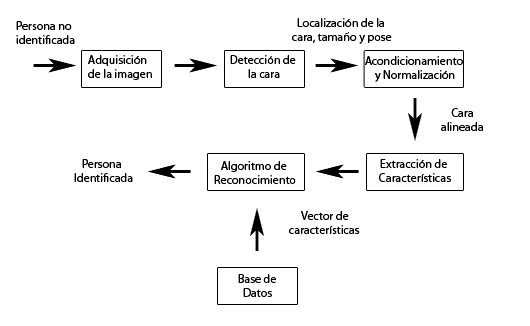
\includegraphics[width=1.3\textwidth]{ML2.png}
 	\end{column}
 	\begin{column}{0.3\textwidth}
 		\centering
 		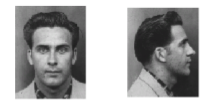
\includegraphics[width=0.6\textwidth]{ML0.png}
 	\end{column}
 	\begin{column}{0.25\textwidth}
 	\centering
 	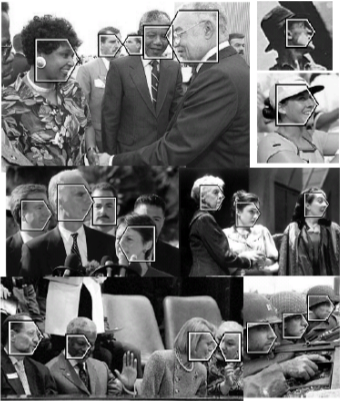
\includegraphics[width=1.1\textwidth]{ML1.png}	
 	\end{column}
 	​  \end{columns}
	
}
\end{frame}
\begin{frame}{\textbf{\textcolor{violet}{Clasificaci\'on: Desde datos a clases discretas}} }
	\vspace{0.2cm}
	
	\textbf{T\'ecnicas de reconocimiento facial}
	
	\scriptsize{ El reconocimiento facial aprovecha la visi\'on artificial para extraer informaci\'on discriminada de im\'agenes faciales y reconocimiento de patrones o t\'ecnicas del machine learning para modelar la apariencia de las caras y para clasificarlas. Por ejemplo:
		
	
		
	\begin{itemize}
		\item SVM
		\item \'Arboles de decisi\'on.
		\item M\'etodos de ensamblado.
		\item Redes neuronales profundas.
	\end{itemize}
	
De wikipedia:

El reconocimiento facial tridimensional, utiliza im\'agenes $3D$ tanto en el entrenamiento como en el reconocimiento. Esta t\'ecnica utiliza sensores en $3D$ para captar informaci\'on sobre la forma de la cara. Se utiliza un derivado del $PCA$ parcial, llamado, \textcolor{orange}{partial principal components analysis}.
}

\end{frame}

\begin{frame}{\textbf{\textcolor{violet}{Clasificaci\'on: Desde datos a clases discretas}} }
	\vspace{0.2cm}
	
	\textbf{Predicci\'on del tiempo}
	
	\scriptsize{No existen solamente procedimiento que recurren  \'unicamente a los modelos meteorol\'ogicos y climatol\'ogicos desarrollados para predecir el tiempo.
		
	\centering
	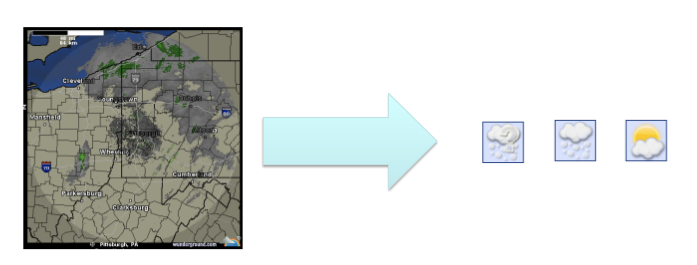
\includegraphics[width=0.8\textwidth]{ML3.png}	
	
 T\'ecnicas del machine learning, incluyendo modelos f\'isicos y redes neuronales profundas  empleando datos  hist\'oricos de las distintas variables meteorol\'ogicas (presi\'on atmosf\'erica, temperatura, punto de roc\'io, campo de vientos, etc) y de situaciones meteorol\'ogicas anteriores, para con los datos recabados en el momento presente, realizar previsiones con una buena precisi\'on .
	}
\end{frame}
\begin{frame}{\textbf{\textcolor{blue}{Regresi\'on que predice un valor num\'erico}}}
\vspace{0.2cm}
	
\textbf{Bolsa de valores}
	
\scriptsize{Una de las formas tanto en condiciones adversas, como en momentos normales en el mercado de predecir hacia donde ir\'a la bolsa as\'i como cada uno de sus valores se llama \texttt{\textcolor{violet}{an\'alisis t\'ecnico}}.

\vspace{0.3cm}

\centering
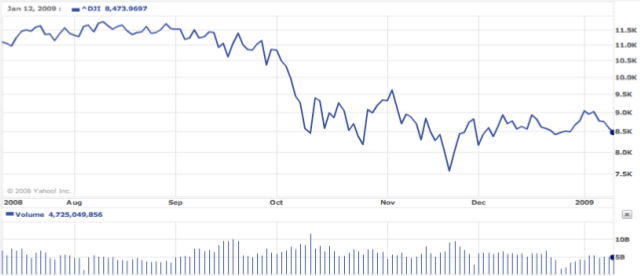
\includegraphics[width=0.65\textwidth]{ML4.png}	

\vspace{0.3cm}
	
El an\'alisis t\'ecnico es un  estudio  de indicadores que se  presentan de forma gr\'afica informaci\'on b\'asica muy necesaria con el objetivo final de tomar una decisi\'on a corto plazo de compra o venta en esas acciones.}
\end{frame}

\begin{frame}{\textbf{\textcolor{blue}{Regresi\'on que predice un valor num\'erico}}}
	\vspace{0.2cm}

\textbf{An\'alisis t\'ecnico y regresi\'on}

\scriptsize{Principalmente el an\'alisis t\'ecnico se basa en un conjunto de operaciones estad\'isticas y matem\'aticas con los precios que van resultando en el mercado, para determinar y detectar situaciones en las tendencias que siguen las cotizaciones de esas acciones a corto y mediano plazo.
	
\begin{itemize}
	\item Econometr\'ia
	\item Matem\'atica financiera avanzada.
\end{itemize}	

El mercado se comporta de una manera gr\'afica tal que el an\'alisis t\'ecnico se puede comparar con un conjunto modelo de variables en las que intentamos predecir el comportamiento futuro con una recta de regresi\'on del tipo simple: $Y= a + bX$.

Es una forma muy b\'asica de predicci\'on, pero es la m\'as cercana a una explicaci\'on matem\'atica simple de c\'omo se realizan las predicciones de los futuros valores burs\'atiles.
}
	
\end{frame}

\begin{frame}{\textbf{\textcolor{blue}{Regresi\'on que predice un valor num\'erico}}}
	\vspace{0.2cm}
	
	\textbf{Predicci\'on del tiempo}
	
\scriptsize{La predicci\'on meteorol\'ogica ha sido tradicionalmente realizada por modelos f\'isicos de la atm\'osfera, que son inestables a las perturbaciones, y por lo tanto son imprecisos para grandes per\'iodos de tiempo. Las t\'ecnicas del machine learning son m\'as robustas a las perturbaciones,  por lo que  generan potencialmente pron\'osticos meteorol\'ogicos m\'as precisos durante grandes per\'iodos de tiempo.
	
\vspace{0.3cm}

\centering
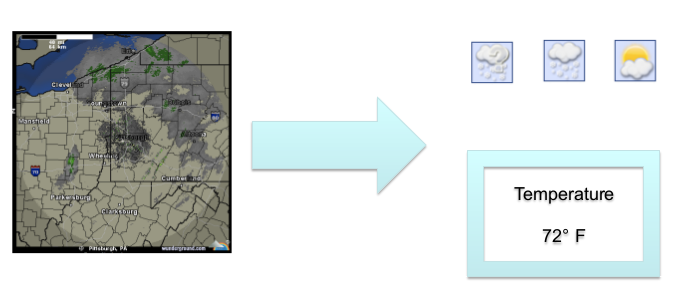
\includegraphics[width=0.7\textwidth]{ML5.png}	

En este contexto, podremos encontrar el valor de la temperatura en determinado escenario, utilizando regresi\'on lineal.}
\end{frame}


\begin{frame}{\textbf{\textcolor{green!55!blue}{Ranking: Comparaci\'on de cosas}}}

	
\textbf{?` Qu\'e es la ingenier\'ia de relevancia?}

\scriptsize{
La \textbf{ingenier\'ia de relevancia} es el proceso de identificar las caracter\'isticas m\'as importantes del conjunto de documentos para los usuarios de esos documentos y utiliza esas caracter\'isticas para afinar el motor de b\'usqueda para devolver los documentos que mejor se adapten a cada usuario en cada b\'usqueda.
 
Para recapitular c\'omo funciona un motor de b\'usqueda: los documentos en tiempo de \'indices se analizan en tokens; estos tokens se insertan entonces en un \'indice como se ve en la figura:

\begin{center}
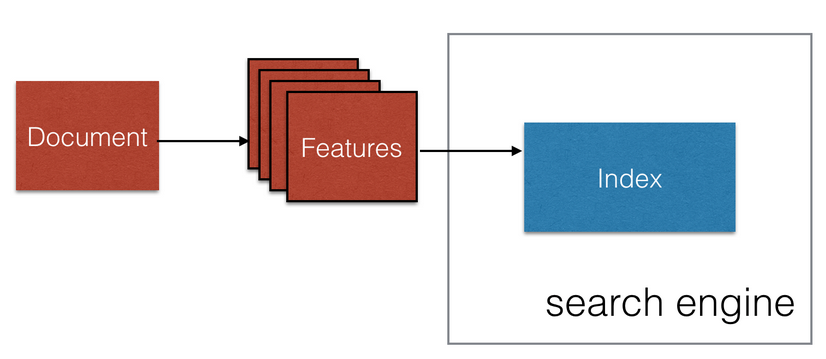
\includegraphics[width=0.6\textwidth]{ML9.png}		
\end{center}
}
\end{frame}

\begin{frame}{\textbf{\textcolor{green!55!blue}{Ranking: Comparaci\'on de cosas}}}
	
\textbf{Funcionamiento de una m\'aquina de b\'usqueda} 

\vspace{0.2cm}

\scriptsize{En el tiempo de b\'usqueda, las consultas individuales tambi\'en se analizan en tokens. El motor de b\'usqueda busca los tokens de la consulta en el \'indice invertido (\textcolor{purple}{inverted index}), clasifica los documentos coincidentes, recupera el texto asociado con esos documentos y devuelve los resultados clasificados al usuario, como se mostrar\'a en la siguiente figura.
	


	
\begin{center}
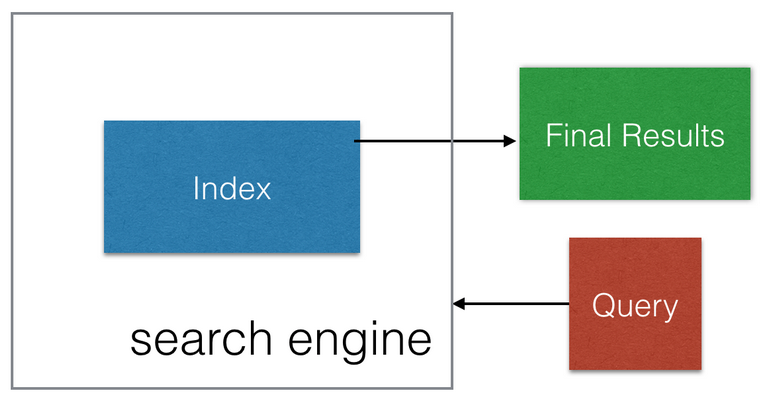
\includegraphics[width=0.55\textwidth]{ML10.png}	
\end{center}


}
\end{frame}

\begin{frame}{\textbf{\textcolor{green!55!blue}{Ranking: Comparaci\'on de cosas}}}
	
\textbf{LTR}

\scriptsize{
	
El \textbf{LTR} aplica el Machine Learning para construir modelos de clasificaci\'on para sistemas de recuperaci\'on de informaci\'on.


Esto significa que en vez de reemplazar el motor de b\'usqueda por un modelo de Machine Learning, estamos ampliando el proceso con un paso adicional. Despu\'es de que se emita la consulta al \'indice, los mejores resultados de esa consulta se pasan al modelo y se vuelven a ordenar antes de ser devueltos al usuario, como se ve en la siguiente figura:

\begin{center}
	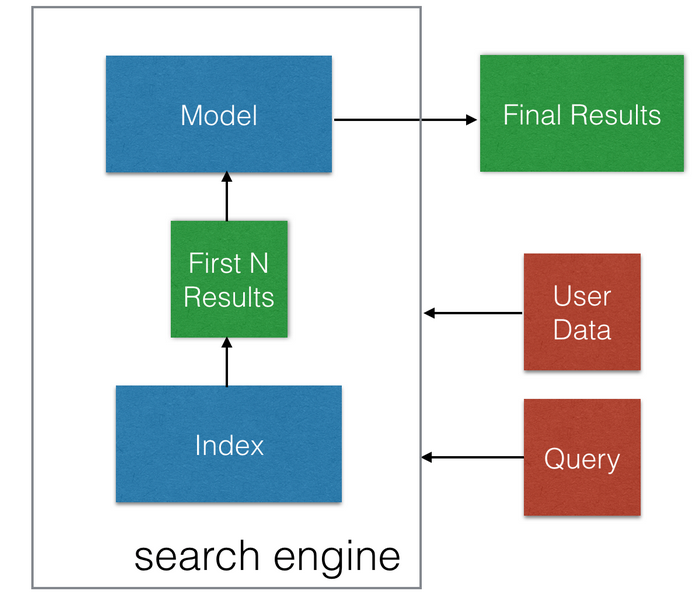
\includegraphics[width=0.4\textwidth]{ML11.png}	
\end{center}
}	
	
\end{frame}

\begin{frame}{\textbf{\textcolor{green!55!blue}{Ranking: Comparaci\'on de cosas}}}
	

\scriptsize{ Learning to Rank  (LTR) es una clase de t\'ecnicas que aplican el machine learning  para resolver \textbf{problemas de ranking}. La principal diferencia entre el  \textcolor{blue}{LTR} y \textcolor{yellow}{ML} tradicional supervisado es la siguiente:


\begin{itemize}
\item El \textcolor{yellow}{ML} tradicional resuelve un problema de predicci\'on (clasificaci\'on o regresi\'on) en una sola instancia a la vez. Por ejemplo, si estas realizando detecci\'on de spam en el correo electr\'onico, ver\'a todas las caracter\'isticas asociadas con ese correo electr\'onico y lo clasificar\'a como spam o no. El objetivo del \textcolor{yellow}{ML} tradicional es llegar a una clase (spam o no spam) o una sola puntuaci\'on num\'erica para esa instancia.

\item El \textcolor{blue}{LTR} resuelve un problema de rankings en una lista de elementos. El objetivo de estas t\'ecnicas es llegar a un ordenamiento \'optimo de esos elementos. Como tal, \textcolor{blue}{LTR} no le importa mucho acerca de la puntuación exacta que cada elemento obtiene, pero se preocupa m\'as por el orden relativo entre todos los elementos. 

\vspace{0.2cm}

Algunos algoritmos \textcolor{blue}{LTR} son: \textcolor{orange}{AdaRank}, \textcolor{brown}{RankCosine}, \textcolor{purple}{IntervalRank}, etc.

\end{itemize}
	
}
\end{frame}
\begin{frame}{\textbf{\textcolor{red}{Filtrado colaborativo y basado en contenido}}}
\textbf{Recomendadores y tipos de filtros}

\vspace{0.2cm}

\scriptsize{Un \textcolor{blue}{recomendador} es un sistema que selecciona un producto que, si se compra, maximiza el valor tanto para el comprador como para el vendedor en un determinado momento del tiempo. 
	
Los recomendadores habitualmente son de dos tipos: los \textcolor{orange}{filtros colaborativos} y los \textcolor{violet}{filtros  basados en contenido}. En este contexto, un filtro es el algoritmo matem\'atico que decide cu\'al es la recomendaci\'on \'optima basado en los datos que le entreguemos.

\begin{itemize}
	\item Los filtros colaborativos generalmente basan su l\'ogica en las caracter\'isticas del usuario. Los datos que se tienen del usuario se convierten en el centro de un filtro colaborativo. Ejemplo: \href{https://www.reddit.com/}{reddit}, \href{https://www.youtube.com}{youtube}  y \href{https://www.last.fm/}{Last.fm}.
	
	\item Los filtros basados en contenido tienen el producto como base de la predicci\'on, en lugar de tener al usuario. Es decir, utiliza las caracter\'isticas del art\'iculo para hacer las recomendaciones. Ejemplo: \href{http://www.imdb.com/}{IMDb} o \href{https://www.rottentomatoes.com/}{Rotten Tomatoes}.
\end{itemize}  }
\end{frame}

\begin{frame}{\textbf{\textcolor{red}{Filtrado colaborativo }}}

\textbf{Algoritmos}

\begin{itemize}
	\scriptsize{
	\item Algoritmos de filtrado colaborativo basados en memoria, o algoritmos de vecinos cercanos(Nearest Neighbour).
}
\scriptsize{
\item Algoritmos de filtrado colaborativo basados en Modelo. Clustering o redes neuronales como las Redes de Funciones de Base Radial (RBFN).}
\end{itemize}

\vspace{0.2cm}

\scriptsize{Un sistema de recomendaciones es mucho m\'as que un algoritmo o un filtro que selecciona productos con m\'as o menos acierto. Podemos dividir un recomendador en $4$ partes: }

\begin{itemize}
	\item La base de conocimiento (la informaci\'on, los datos).
	\item El procesamiento de la base de conocimientos (tecnolog\'ia, algoritmos, filtros).
	\item Anal\'itica y control de negocio (medir todo, estrategia de negocio).
	\item Interface del usuario.
\end{itemize}	
	
\end{frame}

\begin{frame}{Agrupamiento: descubrimiento estructuras en los datos}

\textbf{El problema del agrupamiento}

\scriptsize{El  problema  del  agrupamiento  puede  definirse  como  sigue:  dados  $n$  puntos  en  un   espacio  n-dimensional   particionar  los  mismos  en  $k$  grupos  tales  que  los  puntos  dentro de un grupo son m\'as similares que cada uno a los de los otros grupos, dicha similaridad   se   mide   atendiendo   a   alguna   funci\'on   distancia   (funci\'on   de   disimilaridad) o alguna funci\'on de similaridad.
	
El conocimiento de los grupos puede permitir una descripci\'on sint\'etica de un conjunto de datos multidimensional complejo.

\vspace{0.2cm}

\begin{center}
	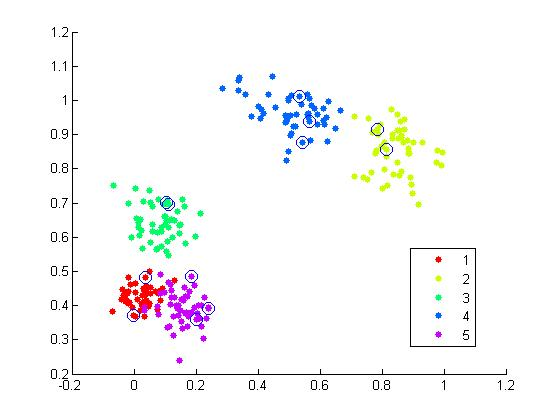
\includegraphics[width=0.45\textwidth]{ML12.png}	
\end{center}	
} 
\end{frame}

\begin{frame}{Agrupamiento: descubrimiento estructuras en los datos}
	
	\textbf{Algoritmos de agrupamiento}
	
	\vspace{0.2cm}
	
	
	\scriptsize{ Existen varias t\'ecnicas para el agrupamiento de casos:
\begin{itemize}		
\item \textcolor{red}{Agrupamiento jer\'arquico}, en los  que se va particionando el conjunto  de  datos  por  niveles, de modo tal que  en  cada  nivel  generalmente , se  unen o se  dividen dos grupos del  nivel anterior ,  seg\'un  si  es  un  algoritmo  aglomerativo  o  divisivo.

\vspace{0.2cm}

Las estrategias jer\'arquicas m\'as conocidas son:

\begin{itemize}
 \scriptsize{\item \textcolor{purple}{Single Link (SL)} En cada paso se unen los dos grupos cuyos elementos m\'as cercanos tienen la m\'inima distancia.}
 \scriptsize{\item \textcolor{orange}{Average Link (AL)} En cada paso se unen los dos grupos tal que tienen la m\'inima distancia promedio entre sus puntos.} 
 \scriptsize{\item  \textcolor{green}{Complete Link (CL)} En cada paso se unen los dos grupos tal que su uni\'on tiene el di\'ametro m\'inimo o los dos grupos con la menor distancia m\'axima entre sus elementos.}
\end{itemize}

\end{itemize}		
}

\end{frame}


\begin{frame}{Agrupamiento: descubrimiento estructuras en los datos}

\begin{itemize}
 \scriptsize{\item \textbf{Chamaleon} Consta de dos fases:}
 	
 	\begin{itemize}
 	\scriptsize	{\item Construye el grafo de los $k$ vecinos m\'as cercanos y  usa un algoritmo de particionamiento de grafo para agrupar los puntos en subgrupos.}
 	\scriptsize {\item Establece   el   par   de   subgrupos   m\'as   similares   considerando interconectividad  y  cercan\'ia usando un algoritmo jer\'arquico aglomerativo.}    
 	\end{itemize}
 	
 \begin{center}
 	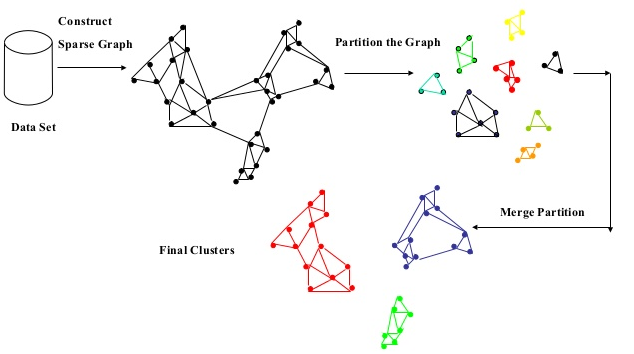
\includegraphics[width=0.45\textwidth]{ML13.png}	
 \end{center}
\end{itemize}
 
\begin{itemize}
	\scriptsize{\item \textcolor{blue}{Agrupamiento no jer\'arquico}, en los que el n\'umero de grupos se determina de antemano y las observaciones se van asignando a los grupos en funci\'on de su cercanía. Por ejemplo el m\'etodo \textcolor{yellow}{k-mean}.
		
}
\end{itemize}
\end{frame}

\begin{frame}{Agrupamiento: descubrimiento estructuras en los datos}
\textbf{k-mean}


\scriptsize{Es uno de los m\'as simples y conocidos algoritmos de agrupamiento, sigue una forma f\'acil y simple para dividir una base de datos dada en $k$ grupos (fijados a priori).
	
La idea principal es definir $k$ centroides (uno para cada grupo) y luego tomar cada punto de la base de datos y situarlo en la clase de su centroide m\'as cercano. El pr\'oximo paso es recalcular el centroide de cada grupo y volver a distribuir todos los objetos seg\'un el centroide m\'as cercano.


El proceso se repite hasta que ya no hay cambio en los grupos de un paso al siguiente.}

 \begin{center}
 	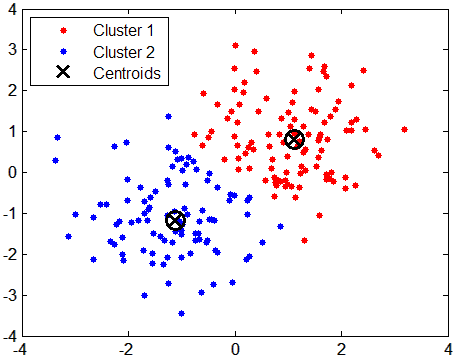
\includegraphics[width=0.35 \textwidth]{ML14.png}	
 \end{center}
 
\end{frame}
\begin{frame}{Agrupamiento: descubrimiento estructuras en los datos}
\begin{itemize}
\scriptsize{\item \textcolor{blue}{Algoritmos basados en densidad}, Estos algoritmos usan diversas t\'ecnicas para determinar dichos grupos las que pueden ser por grafos, basadas en histogramas, kernels, aplicando la \textcolor{orange}{regla k-NN},cempleando los conceptos de punto central, borde o ruido. 
	
Entre ellos podemos mencionar los algoritmos \textcolor{red}{DBSCAN}, \textcolor{green!55!purple}{OPTICS}, \textcolor{purple}{KNNCLUST} y \textcolor{yellow!75!blue}{SNN}
}
\end{itemize}

\vspace{0.3cm}

\begin{center}
	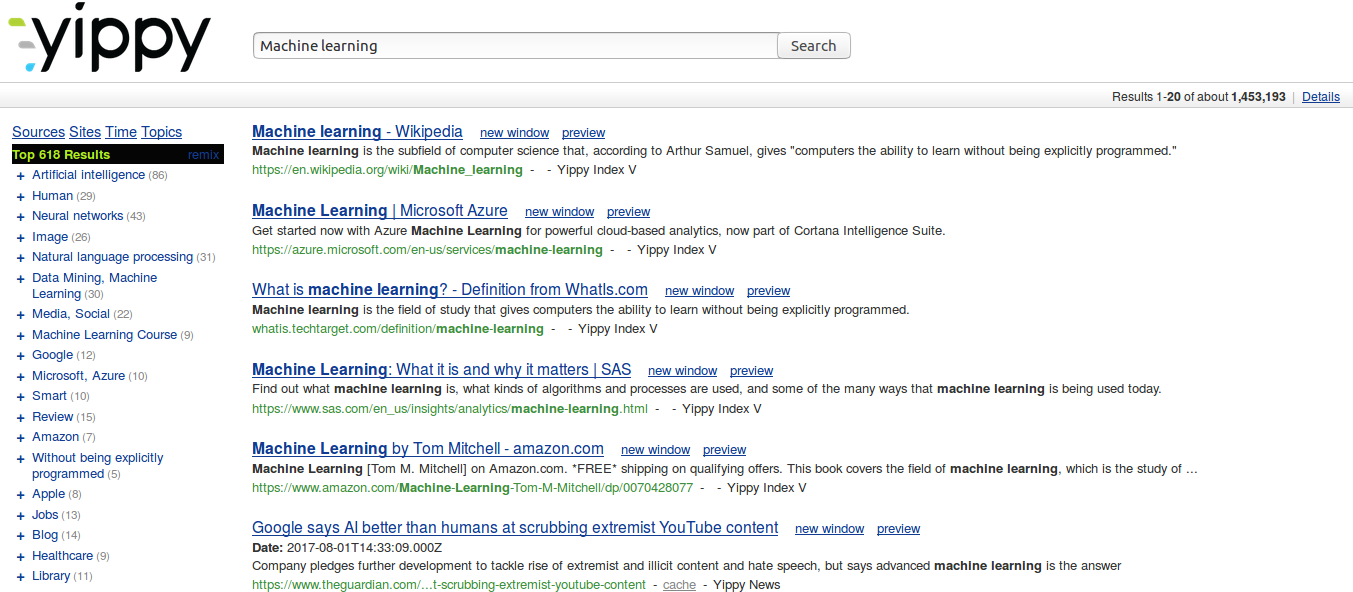
\includegraphics[width=0.7 \textwidth]{ML15.png}	
\end{center}

\vspace{0.3cm}


\tiny{\qquad Clusty es un  metabuscador y  la separaci\'on por categor\'ias de los resultados es buen ejemplo de agrupaci\'on por b\'usqueda web.}

\end{frame}

\begin{frame}{\textbf{\textcolor{green!55!red}{Predicci\'on estructurada de datos a clases discretas}}}
	
\textbf{Redes neuronales y Machine Learning}

\scriptsize{Los sistemas de inteligencia artificial basados en redes neuronales se usan en sistemas de reconocimiento de im\'agenes o, incluso, en los sistemas de dictado de  dispositivos m\'oviles. En el fondo, funcionan de la misma manera que una persona aprende en base a su propia experiencia (y se producen conexiones entre nuestras neuronas cerebrales), una m\'aquina podr\'ia aprender y \texttt{saber qu\'e hacer}  en base a informaci\'on previa (o hist\'orica) suministrada como si fuesen ejemplos (gener\'andose tambi\'en conexiones en la \texttt{red neuronal artificial}).}

\begin{center}
	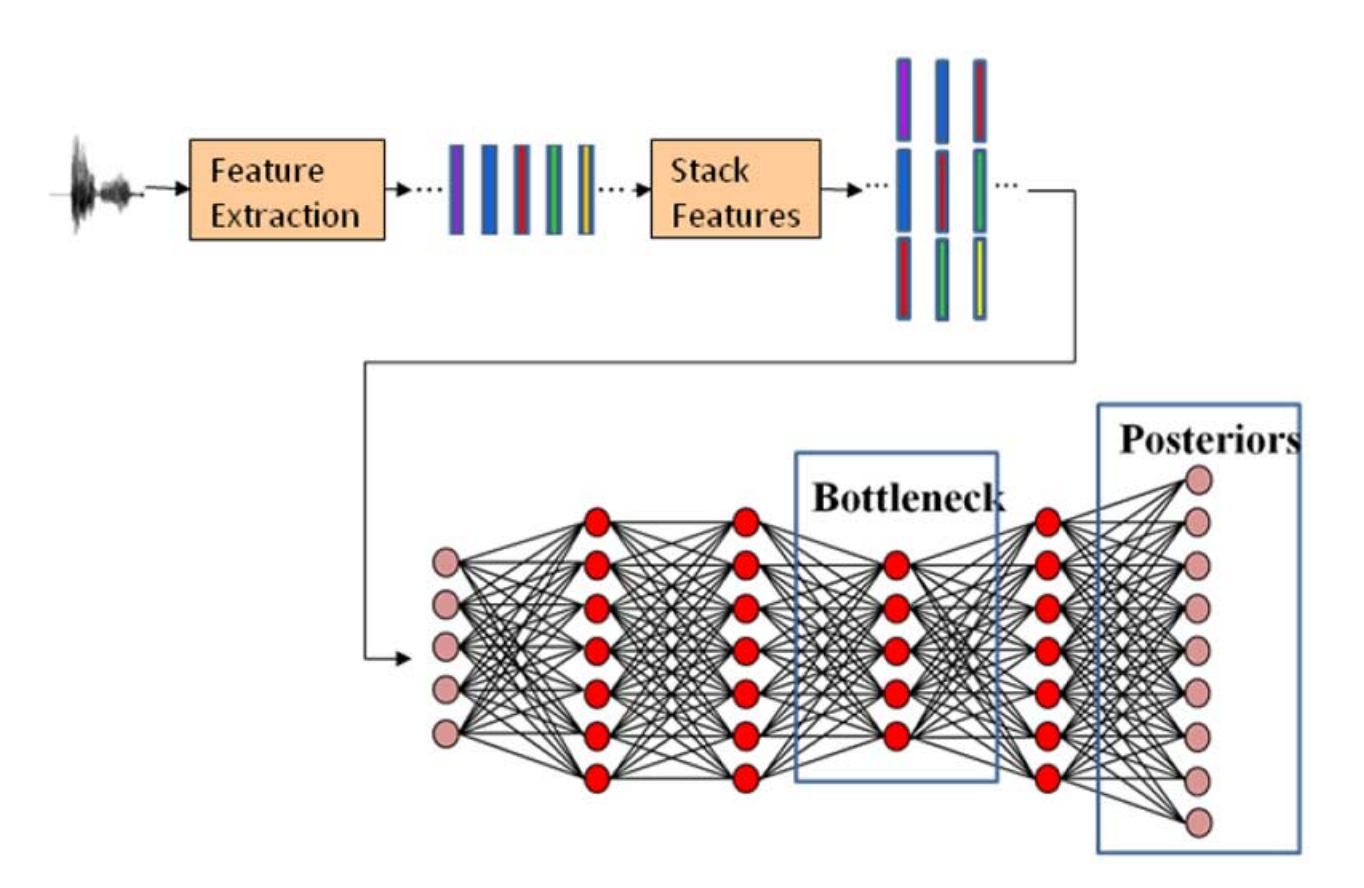
\includegraphics[width=0.6 \textwidth]{ML17.png}	
\end{center}
\end{frame}


\begin{frame}{\textbf{\textcolor{green!55!red}{Predicci\'on estructurada de datos a clases discretas}}}
	
\textbf{Reconocimiento autom\'atico de voz}
	
\scriptsize{Nuestra voz tiene patrones caracter\'isticos como nuestra cadencia a la forma de hablar, las distintas frecuencias que generamos o los fonemas (sonidos que generamos para formar las palabras). 
		
Si un sistema es capaz de aislar estas caracter\'isticas y compararlas con un banco previo de patrones que ya conoce, igual que hace nuestro cerebro, ser\'ia capaz de realizar la identificaci\'on de una voz y asociarla con una persona conocida.  Eso lo puede realizar el Machine Learning con una serie de API's  \href{https://blogs.technet.microsoft.com/machinelearning/2015/12/14/now-available-speaker-video-apis-from-microsoft-project-oxford/}{\textcolor{red}{proyecto Oxford}}.}
	
	\begin{center}
		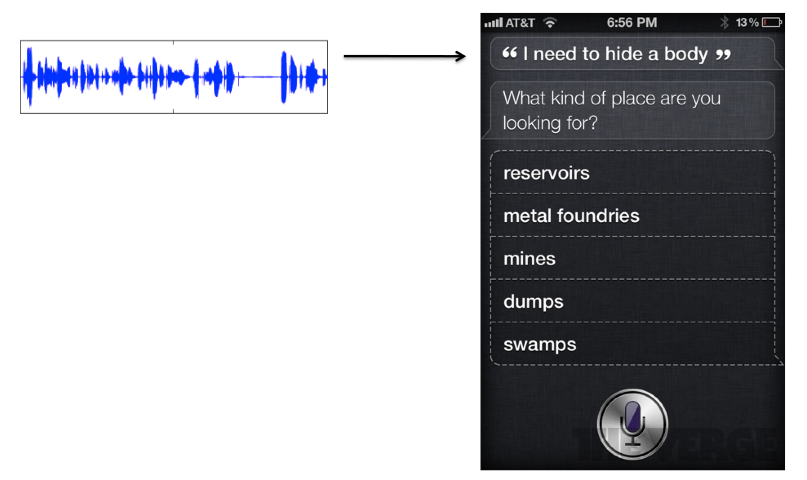
\includegraphics[width=0.55 \textwidth]{ML16.png}	
	\end{center}
\end{frame}


\begin{frame}{\textbf{\textcolor{orange}{Crecimiento del Machine Learning}}}
	\textbf{El machine learning es un enfoque de:}
	\begin{itemize}
		\small{
			\item Reconocimiento de voz, Procesamiento del lenguaje natural.
			\item  Visi\'on por computador
			\item Control de robots
			\item Biolog\'ia computacional
			\item Redes de sensores
			\item \dots
		}
	\end{itemize}
	
	\textbf{Esta tendencia se est\'a acelerando en:}
	\small{
		\begin{itemize}
			\item Big Data
			\item Algoritmos mejorados de Machine Learning
			\item Computadoras m\'as r\'apidas
			\item Buen software de c\'odigo abierto
			\item \dots
		\end{itemize}
	}
\end{frame}

\begin{frame}{\textbf{\textcolor{red}{Mapa del curso}}}
	\textbf{Primera parte: Aprendizaje supervisado}
	
	\begin{itemize}
		\item SVM, m\'etodos del Kernel.
		\item Teoria del aprendizaje.
		\item \'Arboles de decisi\'on, boosting, aprendizaje profundo.
	\end{itemize}
	\textbf{Segunda parte: Ciencia de datos}
	\begin{itemize}
		\item Aprendizaje no supervisado. Algoritmo EM.
		\item Reducci\'on de la dimensi\'on.
	\end{itemize}
\end{frame}

\section{3. Algunos conceptos b\'asicos }

\begin{frame}{Conceptos b\'asicos}
\scriptsize{
	
\begin{itemize}
	\item \textcolor{green!55!purple}{Aprendizaje}: a aquello que la m\'aquina pueda aprender a partir de la experiencia, no a partir del reconocimiento de patrones programados a priori. Por tanto, una tarea central de c\'omo aplicar esta definici\'on al contexto de la computaci\'on va a consistir en alimentar la experiencia de la m\'aquina por medio de objetos con los que entrenarse (ejemplos) para, posteriormente, aplicar los patrones que haya reconocido sobre otros objetos distintos.
\item \textcolor{red}{Machine Learning} en su uso m\'as b\'asico es la pr\'actica de usar algoritmos para parsear datos, aprender de ellos y luego ser capaces de hacer una predicci\'on o sugerencia sobre algo. Dependiendo de los objetos que intentan predecir, podemos tener algunos  tipos de problemas.

\begin{itemize}
\scriptsize{
\item \textcolor{orange}{Regresi\'on:} Intentan predecir un valor real. 
\item \textcolor{blue}{Clasificaci\'on (binaria o multiclase):} Intentan predecir la clasificaci\'on de objetos sobre un conjunto de clases prefijadas. Si solo se permiten $2$ posibles clases, entonces se llama \textcolor{violet}{clasificaci\'on binaria}; si se permiten m\'as de $2$ clases, estamos hablando de \textcolor{violet}{clasificaci\'on multiclase}.
\item \textcolor{blue!75!purple}{Ranking:} Intentar predecir el orden óptimo de un conjunto de objetos según un orden de relevancia predefinido. 
}
\end{itemize} 
\end{itemize}
		}
\end{frame}
\begin{frame}{Conceptos b\'asicos}
\scriptsize{Dependiendo del tipo de salida que se produzca y de c\'omo se aborde el tratamiento de los ejemplos, los diferentes algoritmos de Machine Learning se pueden agrupar en:
\begin{itemize}
\item \textbf{\textcolor{blue}{Aprendizaje supervisado:}} se genera una funci\'on que establece una correspondencia entre las entradas y las salidas deseadas del sistema, donde la base de conocimientos del sistema est\'a formada por ejemplos etiquetados a prior.

\item \textbf{\textcolor{green!45!orange}{Aprendizaje no supervisado:}} donde el proceso de modelado se lleva a cabo sobre un conjunto de ejemplos formados \'unicamente por entradas al sistema, sin conocer su clasificaci\'on correcta. Por lo que se busca que el sistema sea capaz de reconocer patrones para poder etiquetar las nuevas entradas.

Un algoritmo de aprendizaje sin supervisar es organizar los datos de alguna manera o describir su estructura. Esto puede significar agruparlos en cl\'usteres o buscar diferentes maneras de examinar datos complejos para que parezcan m\'as simples o m\'as organizados.

\item \textbf{\textcolor{red}{Aprendizaje por refuerzo:}} en este caso el algoritmo aprende observando el mundo que le rodea y con un continuo flujo de informaci\'on en las dos direcciones (del mundo a la m\'aquina, y de la m\'aquina al mundo) realizando un proceso de ensayo-error, y reforzando aquellas acciones que reciben una respuesta positiva en el mundo.
		\end{itemize}
	}
	\end{frame}
	
\begin{frame}{\textcolor{red}{Consideraciones al elegir un algoritmo}}
\begin{itemize}
\scriptsize{\item \textbf{Precisi\'on:} Se pueden usar m\'etodo m\'as aproximados y reducir el tiempo de procesamiento. Estos m\'etodos tienen a evitar el \textcolor{green}{sobreajuste}. 

\item \textbf{Linealidad}

Muchos algoritmos de ML hacen uso de la linealidad. Los algoritmos de clasificaci\'on lineal suponen que las clases pueden estar separadas mediante una l\'inea recta (o su an\'alogo de mayores dimensiones). }.


\begin{center}
		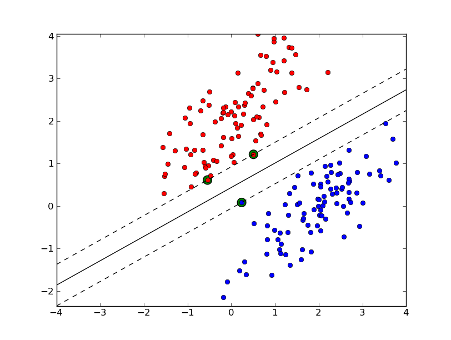
\includegraphics[width=0.45 \textwidth]{ML18.png}	
\end{center}
\item \textbf{Tiempo de entrenamiento:} depende de la precisi\'on. Si el tiempo es limitado, esto puede determinar la elecci\'on del algoritmo, especialmente cuando el conjunto de datos es grande.
\end{itemize}
\end{frame}


\begin{frame}{\textcolor{red}{Consideraciones al elegir un algoritmo}}
\begin{itemize}
\scriptsize{\item \textbf{Cantidad de par\'ametros:}

Los par\'ametros son n\'umeros que afectan al comportamiento del algoritmo, como la tolerancia a errores o la cantidad de iteraciones. 

Normalmente, los algoritmos con par\'ametros de n\'umeros grandes requieren la mayor cantidad de pruebas y errores posibles para encontrar una buena combinaci\'on.

\item \textbf{Cantidad de caracter\'isticas}

Para ciertos tipos de datos, la cantidad de caracter\'isticas puede ser muy grande en comparación con la cantidad de puntos de datos. Este suele ser el caso de la gen\'etica o los datos textuales.

Una gran cantidad de caracter\'isticas puede trabar algunos algoritmos de ML y provocar que el tiempo de entrenamiento sea demasiado largo. Las SVM son especialmente adecuadas para este caso.


\vspace{0.3cm}

Algunos algoritmos de ML hacen determinadas suposiciones sobre la estructura de los datos o los resultados deseados. 
}			
\end{itemize}

\end{frame}
\begin{frame}{\textcolor{green!35!blue}{Notaciones}}
\small{ Usamos $x_i$ para denotar \textcolor{red}{variables de entrada}, tambi\'en llamadas \textcolor{blue}{caracter\'isticas} de entrada y $y_i$ denota la salida o la variable \textcolor{violet}{objetivo}.
	

\vspace{0.2cm}

El par $(x_i, y_i)$ es llamado \textcolor{yellow}{ejemplo de entrenamiento} y el conjunto de datos que vamos a usar para aprender, una lista de $m$ ejemplos de entrenamiento $\{(x_i, y_i); i = 1, \dots m \}$ es llamado \textcolor{orange}{conjunto de entrenamiento}. Tambi\'en denotaremos $X$  como el espacio de valores de entrada e $Y$ el espacio de valores de salida. 
 

\vspace{0.2cm}

Cuando la variable objetivo que estamos tratando de predecir es continua, llamamos al problema de aprendizaje un problema de \textcolor{green!65!blue}{regresi\'on}. Cuando $y$ puede tomar s\'olo un peque\~no n\'umero de valores discretos, lo llamamos un problema de \textcolor{violet}{clasificaci\'on}.

}

\end{frame}

\begin{frame}{\textcolor{green!35!blue}{Notaciones}}
	
\small{Para describir el problema de aprendizaje supervisado, nuestro objetivo es, dado un conjunto de entrenamiento, aprender una funci\'on $f: X \rightarrow Y$ para que $f(x)$ sea un buen predictor  para el valor correspondiente de $y$. Esta funci\'on $f$ se llama \textcolor{green}{hip\'otesis}. El proceso se ve as\'i por ejemplo:
	
	\begin{center}
		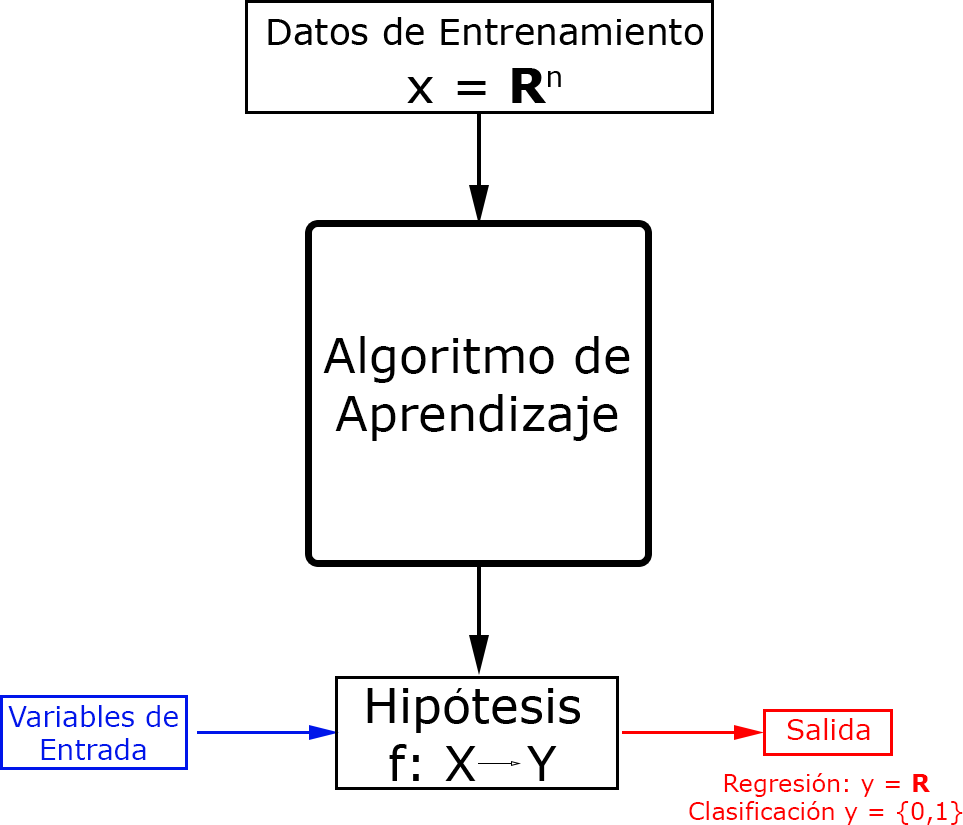
\includegraphics[width=0.42 \textwidth]{ML19.png}	
	\end{center}}
\end{frame}


\begin{frame}{\textbf{\textcolor{violet}{Aprendizaje supervisado: Encuentra $f$}}}
	
\begin{itemize}
	\item \textbf{\textcolor{blue}{Dado:}} Un conjunto de entrenamiento $\{ x_i, y_i	\}|i = 1, \dots, N$
	\item \textbf{\textcolor{blue}{Encuentra:}} Una buena aproximaci\'on a $f: X \rightarrow Y$.
\end{itemize}

\vspace{0.3cm}

 \textbf{\textcolor{blue}{Ejemplos:}}
 
 \begin{itemize}
 	\item \textbf{\textcolor{blue}{Detecci\'on de spam:}}
 	\begin{itemize}
 		\item Mapea email a \{ Spam, no es Spam\}.
 	\end{itemize}
 	\item \textbf{\textcolor{blue}{Reconocimiento de d\'igitos}}
 	\begin{itemize}
 		\item  Mapea pixeles a $\{0,1, 2,3,4,5,6,7,8,9\}$.
 	\end{itemize}
 	\item \textbf{\textcolor{blue}{Predicci\'on de valores}}
 	\begin{itemize}
 		\item   Nuevas funciones, hist\'orico de precios, etc a $\mathbb{R}$ (los n\'umeros reales).
 	\end{itemize}
 \end{itemize}
\end{frame}

\begin{frame}{\textbf{\textcolor{green!55!blue}{Un problema de Aprendizaje supervisado}}}
\begin{columns}
	\begin{column}{0.5\textwidth}
	Conjunto de datos:
	
	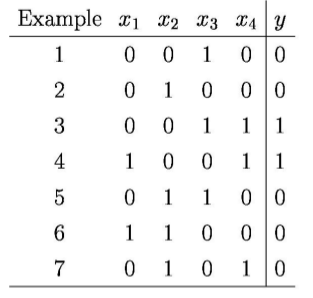
\includegraphics[scale= 0.45]{ML6.png}
	\end{column}
	\begin{column}{0.5\textwidth}  
	\begin{itemize}
		\item Nuestro prop\'osito es encontrar una funci\'on $f: X \rightarrow Y$
		\begin{itemize}
		\item $X = \{0,1\}^4$
		\item $Y = \{0, 1\}$
		\end{itemize}
	\item \textbf{\textcolor{blue}{Pregunta 1}} ?`C\'omo elegir el espacio de  hip\'otesis, el conjunto de funciones posibles $f$?
	\item \textbf{\textcolor{blue}{Pregunta 2}}?` C\'omo encontramos el mejor $f$ en el espacio de  hip\'otesis? 
	\end{itemize}
	\end{column}
\end{columns}
\end{frame}

\begin{frame}{\textbf{\textcolor{red!55!green}{Espacio de hip\'otesis general}}}
Considere todas las posibles funciones booleanas sobre cuatro caracter\'isticas de entrada.

\vspace{0.2cm}

	\begin{columns}
		\begin{column}{0.4\textwidth}
			\begin{itemize}
				\item $2^{16}$ posibles hip\'otesis
				\item $2^9$ son consistente con nuestro conjunto de datos
				\item ?`C\'omo elegimos el mejor?
			\end{itemize}
		\end{column}
		\begin{column}{0.3\textwidth}  
		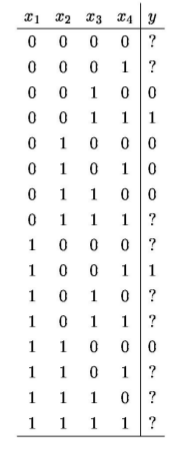
\includegraphics[scale= 0.4]{ML7.png}
		\end{column}
		
		\begin{column}{0.3\textwidth}  
		Conjunto de datos:
		
		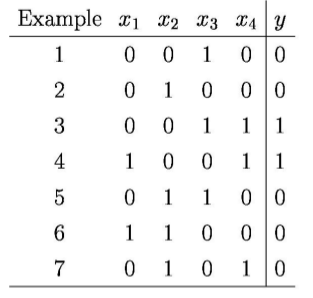
\includegraphics[scale= 0.25]{ML6.png}	
		\end{column}
	\end{columns}
\end{frame}

\begin{frame}{\textbf{\textcolor{blue!55!yellow}{Espacio de hip\'otesis restringido}}}
Considera todas las funciones booleanas conjuntivas.
	
	\vspace{0.2cm}
	
	\begin{columns}
		\begin{column}{0.35\textwidth}
			\begin{itemize}
				\item $16$ posibles hip\'otesis
				\item Ninguno es consistente con nuestros datos
				\item ?`C\'omo elegimos el mejor?
			\end{itemize}
		\end{column}
		\begin{column}{0.4\textwidth}  
			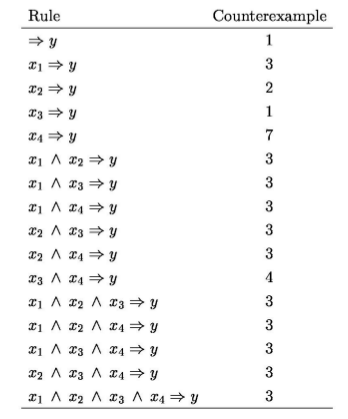
\includegraphics[scale= 0.35]{ML8.png}
		\end{column}
		
		\begin{column}{0.3\textwidth}  
			Conjunto de datos:
			
			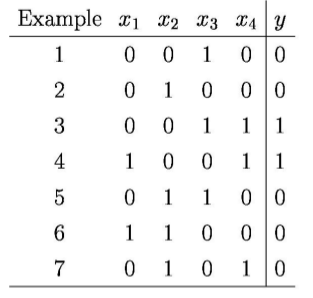
\includegraphics[scale= 0.2]{ML6.png}	
		\end{column}
	\end{columns}
\end{frame}



\begin{frame}{\textbf{\textcolor{green!55!blue}{Principio de la navaja de Ockham}}}

\begin{itemize}
\small{
\item  Guillermo de Ockham, fue un monje que vivi\'o en los a\~nos $1280-1349$.
\item Principio de parsimonia:}

\scriptsize{\texttt{No se debe aumentar, m\'as all\'a de lo necesario, el n\'umero de entidades necesarias para explicar cualquier cosa}}

\small{
\item Cuando hay \textcolor{red}{muchas} soluciones disponibles para un problema dado, debemos seleccionar la m\'as \textcolor{red}{simple}. Pero, ?`qu\'e entendemos por \textcolor{red}{simple}?

\item Usaremos el \textcolor{red}{conocimiento previo (prior)} del problema para resolver para definir lo que es
una soluci\'on simple.

\centering
\scriptsize{\texttt{Ejemplo de un prior: smoothness}}
}
\end{itemize}
\end{frame}

\begin{frame}{\textbf{\textcolor{blue}{Aspectos claves del Machine Learning}}}
	
\begin{itemize}
\small {
	\item  ?`C\'omo elegimos un espacio de hip\'otesis?}
	\begin{itemize}
	\scriptsize{
	\item Con frecuencia utilizamos el conocimiento previo para guiar esta elecci\'on.
}
	\end{itemize}
	\item \small {?`C\'omo podemos medir la exactitud de una hip\'otesis sobre datos nuevos?}
	\begin{itemize}
		\scriptsize{
		\item \textbf{Principio de la navaja de Ockham}: utiliza la hip\'otesis m\'as simple compatible con los datos!.Esto nos ayudar\'a a evitar el sobreajuste.
		\item \textbf{La teoria del aprendizaje} nos ayudar\'a a cuantificar nuestra capacidad de generalizar como una funci\'on de la cantidad de datos de entrenamiento y el espacio de hip\'otesis.
	}
	\end{itemize}
\small {\item ?`C\'omo encontramos la mejor hip\'otesis?}
	 \begin{itemize}
	\scriptsize{\item Esta es una pregunta algor\'itmica, el tema principal de la ciencia de la computaci\'on.}
\end{itemize}
\small {\item ?` C\'omo modelar aplicaciones como problemas de Machine Learning?
(desaf\'io de la  ingenier\'ia)
} 
\end{itemize}
	
\end{frame}
\end{document}